\section{Eliza Petrycka}
\label{sec:Eliza}

Moje ulubione zwierzę (figure~\ref{fig:pletwal}).

\begin{figure}[htbp]
    \centering
    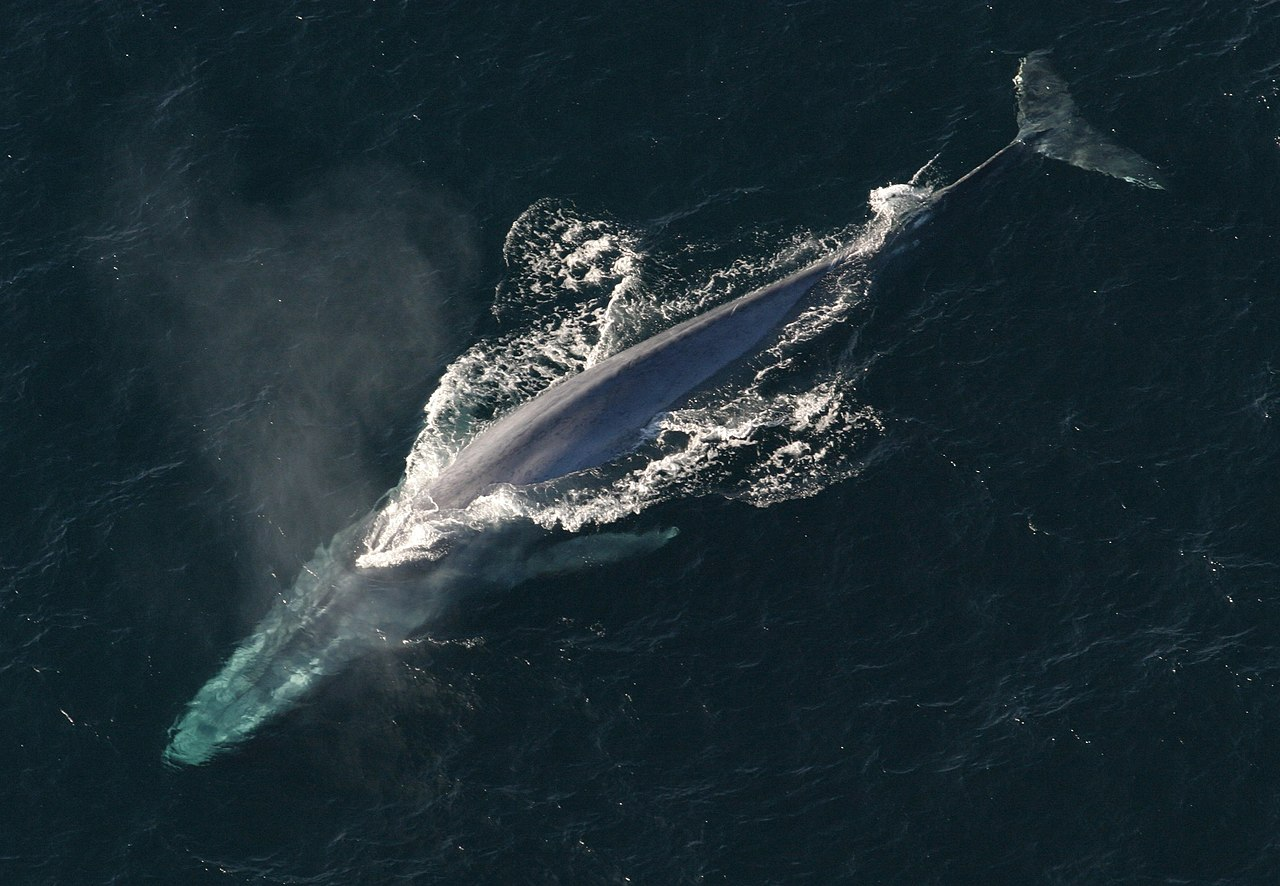
\includegraphics[width=0.3\textwidth]{pictures/eliza.jpg}
    \caption{To jest płetwal}
    \label{fig:pletwal}
\end{figure}

Tabelka~\ref{tab:tabelka_elizy} występowanie płetwali$^1$:
\begin{table}[htbp]
\centering
\begin{tabular}{||l|p{6cm}||} 
\hline
Nazwa potoczna & miejsce występowania\\ [0.5ex] 
\hline
\textbf{płetwal błękitny} &  \fussy{północny Ocean Atlantycki i północny Ocean Spokojny}\\ 
\hline
\textbf{płetwal krótkoogonowy} &  \fussy{Ocean Indyjski i południowo-zachodni Ocean Spokojny wokół Australii}\\
\hline
\textbf{płetwal indyjski} & północny Ocean Indyjski od Somalii po Malediwy\\
\hline
\textbf{płetwal pośredni} & Ocean Południowy\\
\hline
\end{tabular}
\label{tab:tabelka_elizy}
\caption{Jak widać płetwale żyją w oceanach}
\end{table}

Ciekawostki o płetwalach$^1$:
\begin{enumerate}
  \item Samice zwykle są większe od samców.
  \item Język dorosłego płetwala błękitnego waży 2700 kg,
    \begin{itemize}
    \item[*] serce płetwala waży 600 kg,
    \item[*] a warstwa tłuszczowa płetwala ma 0,5 m grubości.
    \end{itemize}
\end{enumerate}

Chociaż mózg wieloryba jest kilkakrtonie większy od naszego to nie potrafi on obliczyć nawet całki: $\int_{x1}^{x2} f(x) \, dx$

\setlength{\parindent}{20pt}

\section*{Krótki tekst}

\textbf{Płetwal} to największe znane zwierzę w historii Ziemi. Jedynym \textit{ naturalnym wrogiem \emph{płetwala jest orka oceaniczna.}}

Dawniej w oceanach żyło wiele osobników płetwala błękitnego. 
\newline
Masowe \underline{polowania }na wieloryby w XX stuleciu sprawiły, że populacja płetwali błękitnych zmniejszyła się \textbf{\textit{wielokrotnie.}}
\footnote{Źródło informacji: Wikipedia}